%%% LaTeX Template: Article/Thesis/etc. with colored headings and special fonts
%%%
%%% Source: http://www.howtotex.com/
%%% Feel free to distribute this template, but please keep to referal to http://www.howtotex.com/ here.
%%% February 2011
%%%
%%% Last updated September 2018 by CDM

%%%  Preamble
\documentclass[11pt,letterpaper]{article}
\usepackage[margin=1.0in]{geometry}
\usepackage[T1]{fontenc}
\usepackage[bitstream-charter]{mathdesign}
\usepackage[latin1]{inputenc}					
\usepackage{amsmath}						
\usepackage{xcolor}
\usepackage{cite}
\usepackage{hyphenat}
\usepackage{graphicx}
\usepackage{float}
\usepackage{subfigure}
\usepackage{sectsty}
\usepackage[compact]{titlesec} 
\usepackage[tablegrid]{vhistory}
\allsectionsfont{\color{accentcolor}\scshape\selectfont}

%%% Definitions
\definecolor{accentcolor}{rgb}{0.0,0.0,0.5} 
\newcommand{\teamname}{Team Name}
\newcommand{\productname}{Product Name}
\newcommand{\coursename}{CSE 4316: Senior Design I}
\newcommand{\semester}{Summer 2019}
\newcommand{\docname}{Project Charter}
\newcommand{\department}{Department of Computer Science \& Engineering}
\newcommand{\university}{The University of Texas at Arlington}
\newcommand{\authors}{Jacob Wilkins \\ Alex Mejia \\ Zohar Moreno \\ Sirjan Khanal \\ Umanga Shrestha}

%%% Headers and footers
\usepackage{fancyhdr}
	\pagestyle{fancy}						% Enabling the custom headers/footers
\usepackage{lastpage}	
	% Header (empty)
	\lhead{}
	\chead{}
	\rhead{}
	% Footer
	\lfoot{\footnotesize \teamname \ - \semester}
	\cfoot{}
	\rfoot{\footnotesize page \thepage\ of \pageref{LastPage}}	% "Page 1 of 2"
	\renewcommand{\headrulewidth}{0.0pt}
	\renewcommand{\footrulewidth}{0.4pt}

%%% Change the abstract environment
\usepackage[runin]{abstract}			% runin option for a run-in title
%\setlength\absleftindent{30pt}			% left margin
%\setlength\absrightindent{30pt}		% right margin
\abslabeldelim{\quad}	
\setlength{\abstitleskip}{-10pt}
\renewcommand{\abstractname}{}
\renewcommand{\abstracttextfont}{\color{accentcolor} \small \slshape}	% slanted text

%%% Start of the document
\begin{document}

%%% Cover sheet
{\centering \huge \color{accentcolor} \sc \textbf{\department \\ \university} \par}
\vspace{1 in}
{\centering \huge \color{accentcolor} \sc \textbf{\docname \\ \coursename \\ \semester} \par}
\vspace{0.5 in}
\begin{figure}[h!]
	\centering
   	
\includegraphics[width=0.60\textwidth]{images/test_image}
\end{figure}
\vspace{0.5 in}
{\centering \huge \color{accentcolor} \sc \textbf{\teamname \\ \productname} \par}
\vspace{0.5 in}
{\centering \large \sc \textbf{\authors} \par}
\newpage


%\vspace{1 in}
%\centerline{January 13th, 2012}
%\newpage

%%% Revision History
\begin{versionhistory}
  	\vhEntry{0.1}{10.01.2018}{GH}{document creation}
  	\vhEntry{0.2}{10.05.2018}{AT|GH}{complete draft}
  	\vhEntry{0.3}{10.12.2018}{AT|GH}{release candidate 1}
  	\vhEntry{1.0}{10.20.2018}{AT|GH|CB}{official release}
  	\vhEntry{1.1}{10.31.2018}{AL}{added customer change requests}
\end{versionhistory}
\newpage

%%% Table of contents
\tableofcontents
\newpage

%%% List of figures and tables (optional)
\listoffigures
%\listoftables
\newpage
\setcounter{table}{0}

%%% Agile project charter sections
\section{Vision}
Most RFID reader kits are complicated and hard to use. This product is being developed to provide RFID reader capabilities to the common user. We want to allow collectors and small businesses to easily keep track of their items. In addition, we'd like to partner with different companies to allow their customers to easily obtain information about their products.

\section{Mission}
To achieve our vision, we will create a cheap, RFID reader that connects an Android phone. We will create a mobile application connected to a database to provide users with information about their items. We will also develop special RFID tags that work with our product.

\section{Success Criteria}
Upon completion of the prototype system, we expect the following success indicators to be observed with clients using our new inventory system:
\begin{itemize}
  \item A 15\% reduction in inventory costs
  \item 20\% reduction in average scanning time
  \item 10\% expansion of the RFID scanning market
\end{itemize}

Within 6 months after the prototype delivery date, we expect the following success indicators to be observed:
\begin{itemize}
  \item An additional 10\% reduction in inventory costs
  \item An additional 10\% reduction in average scanning time
  \item An additional 5\% expansion of the RFID scanning market
  \item Porting the system to iPhone
\end{itemize}

Within 12 months after the prototype delivery date, we expect the following success indicators to be observed:
\begin{itemize}
  \item Expansion of the system to 3 additional deployment sites
  \item Porting of the system to additional mobile platforms
  \item An additional 10\% reduction in inventory costs
\end{itemize}
\\

\newpage

%%% Remaining project charter sections
\section{Background}
The current problem is that our customer has no way to keep track of the inventory or we assume that the inventory is being kept in another form other than digital such as paper which is not a problem but as the production gets bigger makes it more difficult to keep track of the product. Beer that has been already produced needs to be labeled by the date it was produced so that it can be known when is the best time to drink it. As we know, the customer faces the problem of leaving the beer to age too long so they pass their prime time. Another problem being faced is the accommodation of the product, since the production of the beer is made in big quantities a lot of space must be made to accommodate all of it so if it is not accommodated with a system it gets easier to lose track of the oldest or most recent beer therefore taking us back to the previous problem. There are a few options on the market to manage inventory such as online applications, these tend to work very well but have some drawbacks, online inventory must be online at all times otherwise you have no access to the inventory, special bar code scanners must be bought to work with the online inventories because these connect to the internet to the online inventory and also these online inventories work on a memberships basis which in the long run are can cost a significant amount of money. There also exists desktop applications that can just be bought to manage inventories, these are the ones we find in small stores such as Dollar General, Walmart, SAM's Club and many other stores but most of them are targeted to big and more general inventories so they don't really work very well with this kind of small inventory. Another problem for inventory software is that it tends to be very expensive plus some type of bar-code scanner that are also very expensive and for a small inventory like this one of these software would be too much to invest on. The current customer wants a more practicable way to keep track of the inventory without having to spend too much money and easy to use, preferable something that can be done with the help of a smart phone or tablet.to be able to manage the inventory at an inexpensive solution, something that can be easily done with the help of a smart phone.

\section{Related Work}
Discuss the state-of-the-art with respect to your product. What solutions currently exist, and in what form (academic research, enthusiast prototype, commercially available, etc)? Include references and citations as necessary \cite{Rubin2012}. If there are existing solutions, why won't they work for your customer (too expensive, not fast enough, not reliable enough, etc.). This section should occupy 1/2 - 1 full page, and should include at least 5 references to related work.

We want to design a more versatile system that can adapt to small companies and focus more on the adaptability of the software to the needs of the customer so that it can be used in different cases. There are a lot of  solutions for this kind of problem, most of the are commercial since managing inventories has always been a problem, both online and desktop applications are offered.

\textbf{Cin7} is the automated inventory management platform for brands growing their production, it is an online application that requires a monthly fee.
Cin7 integrates the entire product flow from the time it is in the warehouse until it leaves. It can help to run a warehouse much more smoothly since it has a great visibility at all the stages. No need to bother looking around for a product since the Cin7 has a very efficient tracking system.

\textbf{Pros:} The reporting is very well done. It offers a lot of features.

\textbf{Cons:} There is a learning curve, it is not very intuitive so you must learn to use it by reading the documentation.Has an outdated design and it is quite expensive.

\textbf{TradeGecko} is powerful inventory and order management software, it includes intelligent reports and forecasting, manufacturing, a customizable platform plus a mobile sales and inventory app on iPhone and iPad.

\textbf{Pros:} The software is smooth, integrates with the real world and requires minimal training. The inventory management component simplifies inventory management and provides us with all the information we need to manage inventory (no small task).

\textbf{Cons:} Smartphone app is limited. Browser-based software is somewhat slow requiring refreshes for up-to-date stock as well as pretty long loading times during navigation.

\textbf{Finale Inventory} is a cloud inventory software for Warehouse Management. Centralizes your inventory across multiple channels and warehouses. Stock changes made in inventory software gets updated instantly to all added channels.

\textbf{Pros:} Highly Customizable, nearly everything within the software can be customized to the way you want to view it on screen, printed as a report, for search, etc. Easy Copy Paste spreadsheet type updates.

\textbf{Cons:}Coming from a different software previously, there was a steep learning curve as you would expect. Figuring out how you want to customize your screen takes some time as there are just so many features. 

\section{System Overview}
\section{system overview}
image is included here*
This system includes a scanner connected to a computer which is connected to a server which can be accessed by the customers through internet, computers or cellphone apps.

\section{Roles \& Responsibilities}
sirjan

\section{Cost Proposal}
\subsection{Preliminary Budget}
The provided budget is 800 for the project. The team will be using it for buying a RFID scanner, Android smart phone cellphone.The team has decided to invest on a computer to operate for the sole project and store all the necessary data. The team has also decided to buy and use an existing RFID scanner for this project. Since the actual computer and andriod cell phone is not decided we are don't have a exact cost proposal for this project but is estimated to be around the available budget.

\section{Facilities \& Equipment}
Our project is beer Inventory app, which mainly focus on beer arrangement, pricing and keeping track of items and their date etc.  We can test our Inventory app in the brewing lab where there is beer collection. Even we can test our inventory app in the store, hotel to arrange the beer, keeping track of sales and their expiry date. For testing ground, we will check our items in suitable lab which consist of beer collection that can be University, hotels or other places. For marker space it depends we can choose any spaces in University or we can do off Campus, but it should include all the elements (Beer) that we need. Yes, we require specific equipment; as our project is Beer Inventory app we need:
 Scanner
Android phone/Raspberry Pie
 Computer 
First, we will make sure if these items are available in the Lab or not and then we will talk to Prof. Chris Conly. After that what will figure out which will be suitable for us either to purchase or lease, and  we will go with th

\section{Assumptions}
An assumption is a belief of what you assume to be true in the future. You make assumptions based on your knowledge, experience or the information available on hand. These are anticipated events or circumstances that are expected to occur during your project's life cycle.

Assumptions are supposed to be true but do not necessarily end up being true. Sometimes they may turn out to be false, which can affect your project significantly. They add risks to the project because they may or may not be true. For example, if you are working on an outdoor unmanned vehicle, are you assuming that testing space will be available when needed? Are you relying on an external team or contractor to provide a certain subsystem on time? If you are working at a customer facility or deploying on their computing infrastructure, are you assuming you will be granted physical access or network credentials?

This section should contain a list of at least 5 of the most critical assumptions related to your project. For example:

The following list contains critical assumptions related to the implementation and testing of the project.

\begin{itemize}
  \item A suitable outdoor testing location will be available by the 3rd sprint cycle
  \item The X sensing system developed by Sensor Consulting Company will be delivered according to specifications by the 4th sprint cycle
  \item Access to the customer installation site will be provided by the 5th sprint cycle
  \item The customer will provide ample power and network connectivity at the installation site
  \item The installation site network infrastructure will allow TCP network traffic on port 8080
\end{itemize}
\section{Constraints}
The following list contains key constraints related to the implementation and testing of the project.

\begin{itemize}
  \item For the RFID scanner, the total cost should not exceed \$1,000.00.
  \item Due to members of the team having part-time or full-time jobs, an equal amount of tasks have been assigned to each members to have         the protoype finished in time with testing done numerous times to make sure the application is communicating efficiently with the         RFID scanner.
  \item Android application along with the functionality and communication to the RFID scanner must be completed by the first week of             December 2019, which would be from December 1st through December 7th.
  \item The Android application will be developed to meet different versions of Android operating systems out in the market.
  \item The RFID scanner must be able to scan 1D barcodes, which are always found on any beverage product and thus wil make it easy for           the user to scan any 1D barcode from a beverage product.
\end{itemize}

\section{Risks}
This section should contain a list of at least 5 of the most critical risks related to your project. Additionally, the probability of occurrence, size of loss, and risk exposure should be listed. For size of loss, express units as the number of days by which the project schedule would be delayed. For risk exposure, multiply the size of loss by the probability of occurrence to obtain the exposure in days. For example:

The following high-level risk census contains identified project risks with the highest exposure. Mitigation strategies will be discussed in future planning sessions.

\begin{table}[h]
\resizebox{\textwidth}{!}{
\begin{tabular}{|l|l|l|l|}
\hline
 \textbf{Risk description} & \textbf{Probability} & \textbf{Loss (days)} & \textbf{Exposure (days)} \\ \hline
 Availability of andriod cellphone and computer  & 0.50 & 5 & 2 \\ \hline
 Schedules for team meeting  & 0.20 & 14 & 2.8 \\ \hline
 Internet access not available at installation site  & 0.30 & 9 & 2.7 \\ \hline
 Delays in shipping from overseas vendors  & 0.10 & 20 & 2.0 \\ \hline
 Certification delays at compliance testing facility & 0.15 & 10 & 1.5 \\ \hline
\end{tabular}}
\caption{Overview of highest exposure project risks} 
\end{table}

\section{Documentation \& Reporting}
%%% In this section, you will describe all of the various artifacts that you will generate and maintain during the project life cycle. Describe the purpose of each item below, how the content will be generated, where it will be stored, how often it will be updated, etc. Replace the default text for each section with your own description. Reword this paragraph as appropriate.

\subsection{Major Documentation Deliverables}

\subsubsection{Project Charter}
This document will be maintaned using github and will be often updated when the team needs to change certain implications. The initial version will be delivered by September 2019 and final version will be delivered by December 2019

\subsubsection{System Requirements Specification}
This document will be maintaned using github and will be often updated when the team needs to change certain implications. The initial version will be delivered by September 2019 and final version will be delivered by December 2019

\subsubsection{Architectural Design Specification}
This document will be maintaned using github and will be often updated when the team needs to change certain implications. The initial version will be delivered by September 2019 and final version will be delivered by December 2019

\subsubsection{Detailed Design Specification}
This document will be maintaned using github and will be often updated when the team needs to change certain implications. The initial version will be delivered by September 2019 and final version will be delivered by December 2019

\subsection{Recurring Sprint Items}

\subsubsection{Product Backlog}
Items from the SRS will be added to the product backlog in order of importance. We will make decisions on which items to prioritize with a group vote. GitHub will be used to keep an up-to-date version of the product backlog.

\subsubsection{Sprint Planning}
How will each sprint plan be planned? How many sprints will there be (you need to look at the schedules for this course and previous Senior Design II courses during the appropriate semesters to figure this out).

\subsubsection{Sprint Goal}
The spring goal will decided by the group. We will discuss what a reasonable goal will be based on our knowledge and the difficulty of the task. The input from the customer will also be taken in consideration.

\subsubsection{Sprint Backlog}
The team leader will decided what backlog products will make into the sprint backlog. The backlog will be maintained by the team leader in a shared file in Google Drive or GitHub.


\subsubsection{Task Breakdown}
Each individual from the team will list their programming skills and based on that will be given a task to complete. The amount of time that they have to complete will be documented in the sprint as well, also if they find a task that they think it fits their set of skill, they can claim that task for themselves.

\subsubsection{Sprint Burn Down Charts}
The team captain will generate the burndown chart. GitHub will be able to keep track of who completed which tasks. The burndown chart will be an excel graph that keeps track of how many tasks are remaining.

\begin{figure}[h!]
    \centering
    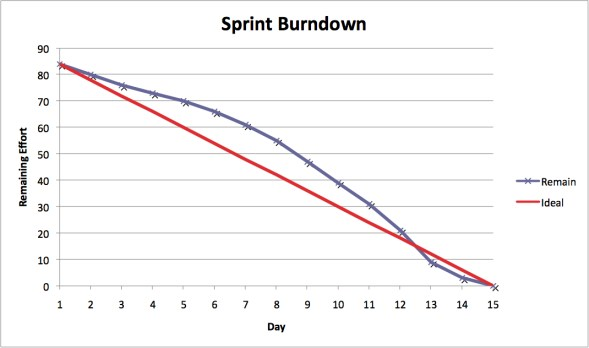
\includegraphics[width=0.5\textwidth]{images/Sprint_Burndown}
    \caption{Example sprint burn down chart}
\end{figure}

\subsubsection{Sprint Retrospective}
The scrum master will meet with the team to discuss what went well and what can be improved on the next sprint. This meeting will happen within a week after each sprint is completed. It will be documented in a sprint retrospective file and turned in December 2019.

\subsubsection{Individual Status Reports}
After each sprint, we are going to report status of the overall development of the application and reports of the functionality and interface between the application and the RFID scanner.  In addition, every week each individual will need to report their status to every team member in the group, that way everyone is up-to-date in the progress of the application and it's functionality with the RFID scanner.  The key items that'll need to be reported are as follows:
1.) Status of GUI development
2.) Testing of different versions of Android operating systems to make sure the application and the RFID scanner interface correctly.
3.) Reports of beverage information safely stored in the database.
4.) Reports of bugs found in the application and fixes applied to the application.
5.) Reports of the condition of the RFID scanner throughout development and testing.
6.) Reports of how much money is being spent on the product.

\subsubsection{Engineering Notebooks}
The engineering notebooks will be updated after each team meeting which will happen, at a minimum, every two weeks. During the two week interval, at least one page of documentation will be completed. Each member will keep track of their on work in their own ENB. At least one other teammate will sign as a witness another teammate in their ENB.


\subsection{Closeout Materials}

\subsubsection{System Prototype}
The system prototype will include a mobile app, an RFID reader, possibly an RFID tag printer, and a database. It will be demonstrated upon completion for the class in December 2019. There will be no Prototype Acceptance Test (PAT) with the customer. Nothing will be demonstrated off-site.

\subsubsection{Project Poster}
The poster will include the product name, team name, team vision, product picture, and key features of the product. It will be presented during the product presentation in December 2019.

\subsubsection{Web Page}
The product web page will include a shop to sell the product and describe the features of the product. In addition, it will describe how the product was designed and why the product was designed. It will be accessible to the public. This will be delivered December 2019. The web page will be completed at closeout.

\subsubsection{Demo Video}
The demo video will include a brief demonstration of the computer screen and smart phone applications working together as well one of our members working with the scanner and label maker. The approximated time will be about 2 - 4 minutes. The topics covered will be the label making, scanning a new product, managing the database from the desktop application.

\subsubsection{Source Code}
The source code will be maintained in GitHub. Both the source code and the executable files will be provided to the customer. All of there will be saved in a cloud service so that it can be downloaded as many times is needed. The source code will be posted in a public repository in GitHub for the general public with a MIT license. The license will be listed in the "read-me" file or its own file.

\subsubsection{Source Code Documentation}
The specific documentation standard will be decided at a later date. We will use Doxygen to document the product. The final documentation will be available in PDF form and HTML form on the product web page.

\subsubsection{Hardware Schematics}
The project is only software.

\subsubsection{CAD files}
The project is only software.

\subsubsection{Installation Scripts}
The mobile application will be sent through GitHub and installed in the device via Android Studio. If any desktop application is developed, it will be provided using a installation script. 

\subsubsection{User Manual}
The customer will be provided with a digital manual and there will also be instructions in the application as well. If the software proves to be more complicated that we think, then a setup video will be created to show the customer how to operate the software and hardware.

\newpage

%%% References
\bibliographystyle{plain}
\bibliographystyle{reference/IEEEtran_custom}
\bibliography{reference/refs}{}

\end{document}
